\section{Solution}\label{sec:solution}

In this part, we present our preliminary solution for achieving fast deadlock-free routing reconfiguration.

During the routing reconfiguration process, to avoid routing blackhole~\cite{everflow} and transient routing loop~\cite{dionysus}, each packet should be forwarded either using the rules prior to the reconfiguration, or the rules after the reconfiguration, but never a mixture of the two. This is called \textit{per-packet consistency}. To implement such an abstraction, a two-phase commit mechanism was proposed~\cite{abstractionforupdate}. This mechanism guarantees atomic configuration of a single path. In our solution, we follow the widely adopted two-phase commit mechanism~\cite{abstractionforupdate,zupdate,dionysus}, and assume the routing reconfiguration is performed at the path level instead of the single rule level.


\subsection{Configuration Dependency Graph}\label{subsec:cdg}

\begin{figure}[t]
	\centering
	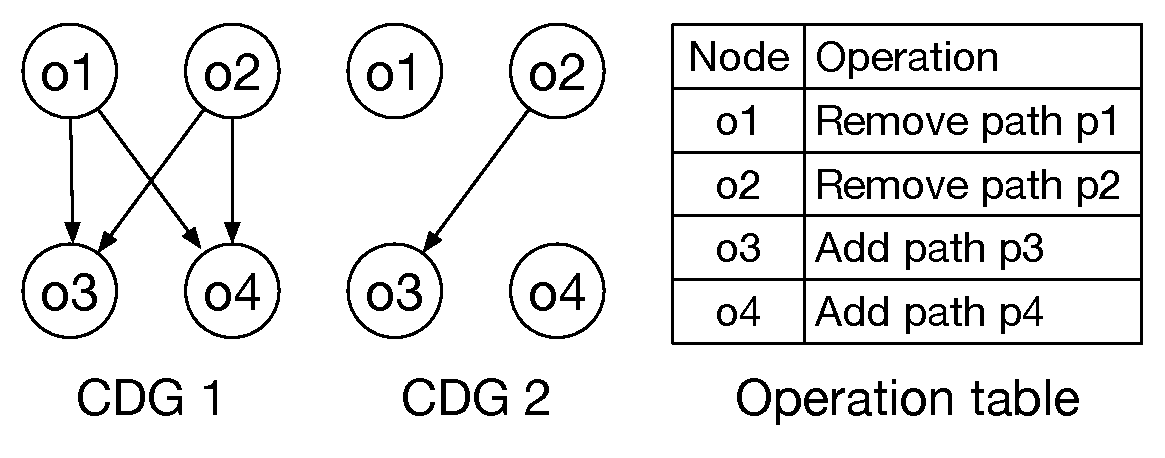
\includegraphics[width=0.45\textwidth] {figs/CDG}
	\caption{Representing the two deadlock-free reconfiguration schemes in Fig~\ref{fig:treecase}(f) using two configuration dependency graphs.}\label{fig:cdg}
	\vspace{-0.15in}
\end{figure}

\begin{figure}[t]
	\centering
	
	\subfloat[short for lof][Topology and path.] {
		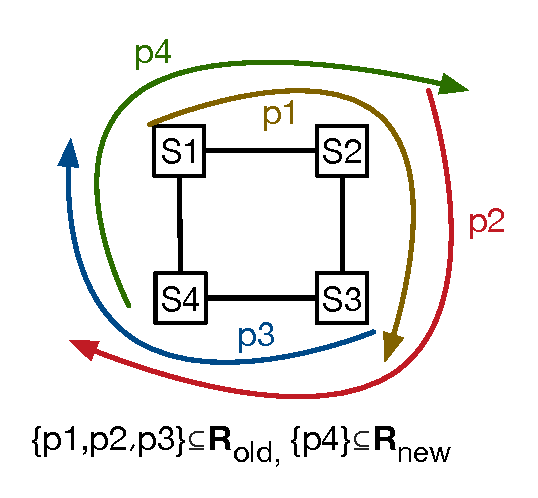
\includegraphics[width=0.22\textwidth] {figs/relationship_or_a}
	}
	\subfloat[short for lof][Deadlock-free scheme and Corresponding CDG.]{
		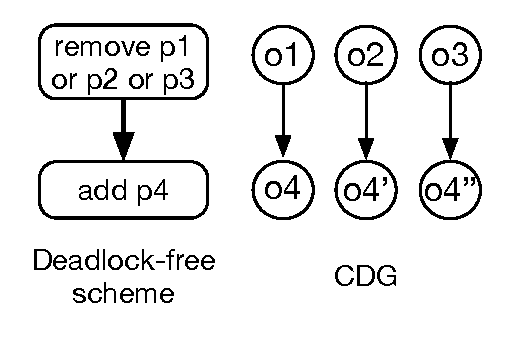
\includegraphics[width=0.24\textwidth] {figs/relationship_or_b}
	}
	
	
	\caption{An example to show the OR relationship. Node $oi$ is the operation to configure path $pi$.}\label{fig:orrelationship}
	\vspace{-0.2in}
\end{figure}

In this part, we define \textit{configuration dependency graph} (CDG) to represent any possible routing reconfiguration schemes at the path level. CDG is a directed graph $G_c(V_c,E_c)$, where each node in $V_c$ represents a configuration operation, and each edge in $E_c$ represents an operation dependency. 

In Fig.~\ref{fig:cdg},  we use two CDGs to represent the two deadlock-free reconfiguration schemes in Fig~\ref{fig:treecase}(f). In the first reconfiguration scheme, it requires paths $p1$ and $p2$ to be removed before paths $p3$ and $p4$ are added, hence we use four edges $o1\rightarrow o3$, $o1\rightarrow o4$, $o2\rightarrow o3$, $o2 \rightarrow o4$ in CDG 1 to capture the order dependencies among operations. In the second reconfiguration scheme, it only requires paths $p2$ to be removed before path $p3$ is added. So only one edge $ o2 \rightarrow o3$ is needed in CDG 2.
 


In order to represent any possible routing reconfiguration schemes, our CDG should be able to describe both the ``OR" and ``AND" relationship that could be used in a reconfiguration scheme, as we are going to explained in the next.

\textbf{OR relationship}: It refers to the dependency relationship that a path can be added after any path in a path set is removed. In Fig.~\ref{fig:orrelationship}, we use an example to illustrate this OR relationship. Fig.~\ref{fig:orrelationship}(a) includes a 4-switch network and four paths $p1$, $p2$, $p3$ and $p4$, where $\{p1, p2, p3\}\subseteq 
R_{old}$ and $\{p4\}\subseteq R_{new}$. In Fig.~\ref{fig:orrelationship}(b), a feasible deadlock-free reconfiguration scheme is presented. In order to avoid cyclic buffer dependency, the scheme requires that at least one path in $\{p1, p2, p3\}$ should be removed before path $p4$ is added. This is the "OR" relationship that could be used in a reconfiguration scheme.

To capture the ``OR" relationship in the CDG, we can duplicate the operation that ``partially" depends on other operations into several mirror operations. As shown in the CDG of Fig~\ref{fig:orrelationship}(b), operation o4 is duplicated into three mirror operations o4, o4' and o4''. Operations $o1$, $o2$ and $o3$ are pointed to different mirror operations of $o4$. During the reconfiguration process, as long as one operation in $\{o1, o2, o3\}$ finishes, the operation to add path $p4$ can start immediately as one of the three mirror operations is released.


\begin{figure}[t]
	\centering
	
	\subfloat[short for lof][Topology and path.] {
		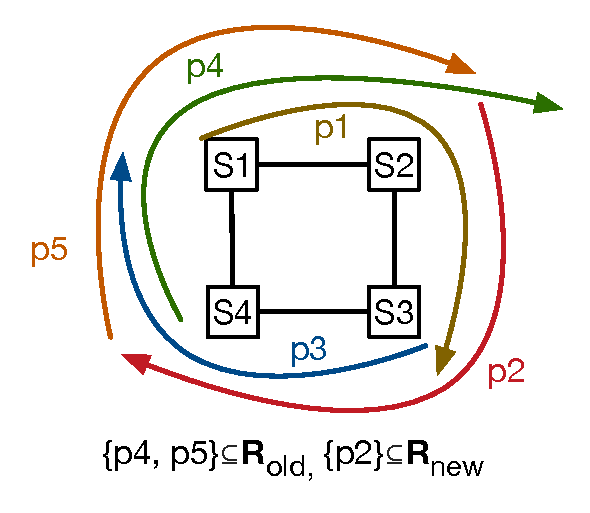
\includegraphics[width=0.24\textwidth] {figs/relationship_and_a}
	}
	\subfloat[short for lof][Deadlock-free scheme and Corresponding CDG.]{
		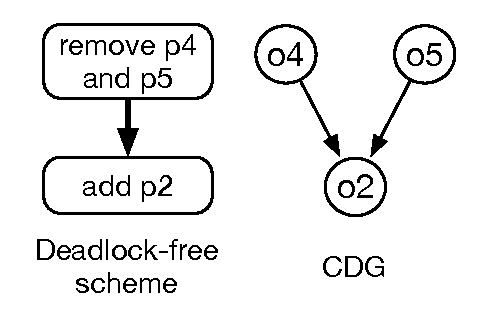
\includegraphics[width=0.24\textwidth] {figs/relationship_and_b}
	}
	
	
	\caption{An example to show the AND relationship. Node $oi$ is the operation to configure path $pi$. }\label{fig:andrelationship}
	\vspace{-0.2in}
\end{figure}

\textbf{AND relationship}: It refers to the dependency relationship that a path can be added after all the paths in a path set are removed. In Fig~\ref{fig:andrelationship}, we use an example to illustrate this AND relationship. As shown in Fig.~\ref{fig:andrelationship}(a), five paths $p1$, $p2$, $p3$, $p4$ and $p5$ traverses a 4-switch network. Both path $p4$ and $p5$ go through S4, S1 and S2 consecutively, but ends at different hosts (not drawn in the figure). In this example, we have $\{p4, p5\}\subseteq R_{old}$ and $\{p2\}\subseteq R_{new}$. Paths $p1$, $p3$ are not involved in the routing reconfiguration.  In Fig.~\ref{fig:andrelationship}(b), a feasible deadlock-free reconfiguration scheme is presented. In order to avoid cyclic buffer dependency, the scheme requires that both of paths $p4$ and $p5$ to be removed before path $p2$ is added. This is the "AND" relationship that could be used in a reconfiguration scheme.

To capture the ``AND" relationship in a CDG, we can let multiple operations point to a single operation, as shown  in the CDG of Fig~\ref{fig:andrelationship}(b). During the reconfiguration process, operation $o2$ will start only after both operations $o4$ and $o5$ finish.

\subsection{Construction of Deadlock-free Configuration Dependency Graph}\label{subsec:dfcdg}

In this part, we present our solution for constructing deadlock-free CDGs. We will also show that if the time to configure a single path can be known in advance or can be accurately estimated, the fastest deadlock-free CDG can be constructed in polynomial time.

Our solution is designed based on the following important observation: \textit{For any cycle in the network, as long as an old buffer dependency edge is permanently removed from the cycle before a different new buffer dependency edge is added to the cycle, there will be no cyclic buffer dependency in the cycle during the routing reconfiguration process.}

This observation can help us to ensure deadlock-free without removing all the paths in $R_{old}$ at first. Before we introduce our solution, we define a few notations used in our solution.

Buffer dependency edges are among ingress queues. As a network link is exactly corresponding to an ingress queue, we use $d_{lx,ly}$ to denote the buffer dependency edge from the ingress queue connected with link $lx$ to the ingress queue connected with link $ly$. We denote a buffer dependency $d_{lx,ly}$ as $d^{o}_{lx,ly}$, if it is created by a path in $R_{old}$. And as $d^{n}_{lx,ly}$ if it is created by a path in $R_{new}$.

We use $D_{o}$ to denote the set of all buffer dependency edges related to the paths in $R_{old}$, and $D_{n}$ to denote the set of all buffer dependency edges related to the paths in $R_{new}$. $O(d^{o}_{lx,ly})$ is the set of operations that can remove the buffer dependency edge $d^{o}_{lx,ly}$ from the network, and $O(d^{n}_{la,lb})$ is the set of operations that can add the buffer dependency edge $d^{n}_{la,lb}$ to the network.



Our solution consists of 3 steps as follows.

\textbf{Step-1: Building $D_{o}$ and $D_{n}$.} We enumerate all the paths in $R_{old}$ and $R_{new}$ to build $D_{o}$ and $D_{n}$. If a buffer dependency edge included in $D_{o}$ is also included in $D_{n}$, we delete it from $D_{o}$ as this edge cannot be permanently removed.

\textbf{Step-2: Constructing a raw deadlock-free CDG.}  For every pair of edges ($d^{o}_{lx,ly}$,  $d^{n}_{la,lb}$), to ensure $d^{o}_{lx,ly}$ is removed from the cycle before  $d^{n}_{la,lb}$ is added to the cycle in the raw CDG, we perform two actions. 

First,  for any operation $oi$ in $O(d^{o}_{lx,ly})$, we create a mirror operation denoted as $oi'$ in the raw CDG. Do the same for any operation $oj$ in $O(d^{n}_{la,lb})$ (denoted as $oj'$).  Second, we add a dependency edge from $oi'$ to $oj'$ for every such pair of operations.

\textbf{Step-3: Deriving deadlock-free CDG(s) from the raw deadlock-free CDG.}  For each connected subgraph in the raw CDG we construct in step-2,  its operation dependency edges ensure that one old buffer dependency edge is permanently removed from a cycle before a new buffer dependency edge is added to the same cycle. This means that each subgraph stand alone can ensure deadlock-free for a certain cycle.  

Assuming the network contains $n$ cycles, a deadlock-free CDG can be created by picking $n$ subgraphs from the raw CDG,  with each subgraph corresponding for a cycle in the network. Different combinations is corresponding to different deadlock-free CDGs.

\textbf{Calculation of fastest deadlock-free CDG}: If the time of any single configuration operation is already known, then we can easily calculate the total configuration time of any subgraph in the raw CDG. In this case, By choosing a subgraph with minimum configuration time for each cycle, we can produce a fastest deadlock-free CDG in polynomial time.

\begin{figure}[t]
	\centering
	
	\subfloat[short for lof][Topology and paths.] {
		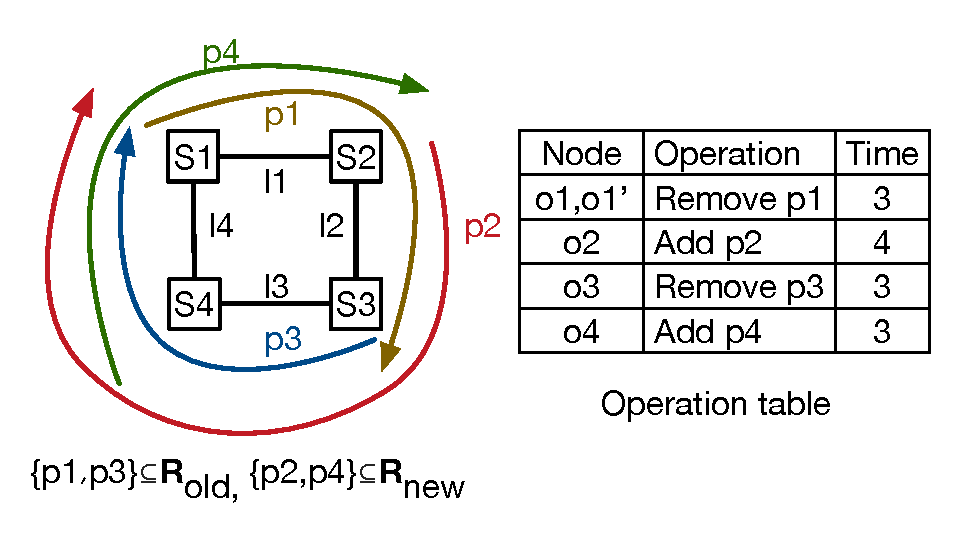
\includegraphics[width=0.26\textwidth] {figs/solution_example_a} 
	}
	\subfloat[short for lof][Raw CDG and Fastest CDG.] {
		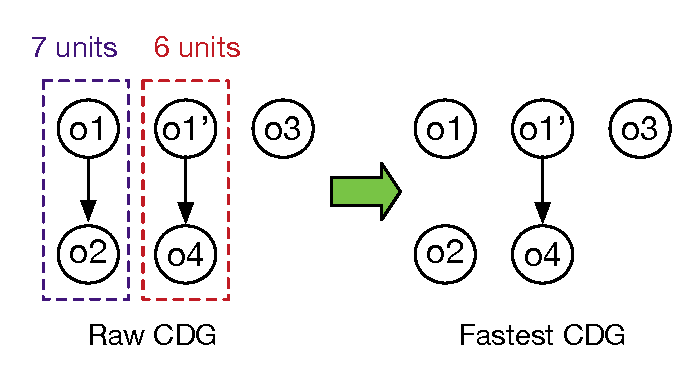
\includegraphics[width=0.22\textwidth] {figs/solution_example_b}
	}
	
	\caption{An example to illustrate the solution. In this example, we simply assume the time cost to configure a path is equal to the number of switches this path traverses.}\label{fig:solution_example}
	\vspace{-0.2in}
\end{figure}

In Fig.~\ref{fig:solution_example}, we have an example to show how our solution works. As shown in Fig.~\ref{fig:solution_example}(a), there are four paths traversing a 4-node network. We have $\{p1, p3\}\subseteq R_{old}$ and $\{p2, p4\}\subseteq R_{new}$. It is easy to calculate $D_{o}=\{d^{o}_{l1,l2},  d^{o}_{l3,l4}\}$, and $D_{n}=\{d^{n}_{l2,l3},  d^{n}_{l3,l4},  d^{n}_{l4,l1}\}$.  According to the algorithm in step-1, $d^{o}_{l3,l4}$ will be deleted from $D_{o}$ as we have $d^{n}_{l3,l4}$ in $D_{n}$.

For all the remaining buffer dependency edges, their corresponding operations are as follows: $O(d^{o}_{l1,l2}) = \{o1\}$, $O(d^{n}_{l2,l3}) = \{o2\}$, $O(d^{n}_{l3,l4}) = \{o2\}$ and $O(d^{n}_{l4,l1}) = \{o4\}$. Then according to step-2, for every pair of edges ($d^{o}_{lx,ly}$,  $d^{n}_{la,lb}$), we create some mirror operations as well as the corresponding dependency edges in the raw CDG. The raw CDG can be found in Fig~\ref{fig:solution_example}(b) (Note that one redundant subgraph $o1'' \rightarrow o2'$ is not drawn).  

As we can find, every connected subgraph in the raw CDG exactly removes one old buffer dependency edge from the cycle before adding a new buffer dependency edge to the  cycle. Hence we can derive two deadlock-free CDGs from the raw CDG: CDG 1 only includes the dependency $o1\rightarrow o2$, while CDG 2 only includes the dependency $o1'\rightarrow o4$.

As shown in Fig.~\ref{fig:solution_example}, if we know the time of any single operation, the total configuration time of any subgraph in the raw CDG can be easily calculated. For example, operations in subgraph $o1 \rightarrow o2$ needs 7 time units to finish, while operations in subgraph $o1' \rightarrow o4$ only needs 6 time units to finish.  Then we can produce a fastest deadlock-free CDG with 6 configuration time, as shown in Fig.~\ref{fig:solution_example}(b).


%\subsection{Fast Deadlock-free Reconfiguration For a Single Cycle}\label{subsec:dfrforsc}
%
%In this part, we present our solution for constructing a deadlock-free CDG $G_c(V_c,E_c)$ for a single topology cycle $C$ in $G(V,E)$. 
%
%The naive approach to find an optimal deadlock-free CDG is to enumerate all the possible CDGs, and choose a deadlock-free CDG with minimum configuration time. However, it would be computationally impossible as there are combinatorial such CDGs. 
%
%Our solution is designed based on the observation that \textit{For a single topology cycle with cyclic buffer dependency, as long as we guarantee that one old buffer dependency edge is removed from the cycle before one different new buffer dependency edge is added to the cycle, the reconfiguration process will be deadlock-free.} 
%
%In the next, we describe how our solution works. For each pair of adjacent links $lx$ and $ly$ in cycle $C$, let $P_s^{lx,ly}$ be the set of paths in $P_s$ contributed to the buffer dependency edge $d_{lx,ly}^{P_s}$, and $P_t^{lx,ly}$ be the set of paths in $P_t$ contributed to the buffer dependency edge $d_{lx,ly}^{P_t}$. Removing all paths in $P_s^{lx,ly}$ will delete buffer dependency edge $d_{lx,ly}^{P_s}$ from the network, while adding paths in $P_t^{lx,ly}$ will create buffer dependency edge $d_{lx,ly}^{P_t}$.
%
%
%For any non-empty set $P_t^{lx,ly}$, as $P_t$ is deadlock-free, there exists at least one 
%
%Given two non-empty sets $P_s^{lx,ly}$ and $P_t^{lm,ln}$ that satisfy $(lx, ly) \neq (lm, ln)$, to guarantee one old buffer dependency edge is removed before one different new buffer dependency edge is added, we can let all the paths in $P_s^{lx,ly}$ be removed from the network before adding any path in $P_t^{lm,ln}$. In other word, we can construct a deadlock-free CDG by adding a configuration dependency edge from any path in $P_s^{lx,ly}$ to any path in $P_t^{lm,ln}$.
%
%In the next, we present our solution for searching deadlock-free CDGs with minimum time cost.  Assuming that we know the time cost to remove or add a single path. Then we can calculate the time cost of path configurations for any $P_s^{lx,ly}$ and any $P_t^{lm,ln}$. To find the optimal CDG(s), our solution will calculate the time cost of path configurations for any legal pair ($P_s^{lx,ly}$, $P_t^{lm,ln}$), and then choose the one with minimum time cost. 
%
%Let $k$ be the number of links in $C$, and $n$ be the number of paths contributed to the buffer dependency in $C$. The time complexity of the above calculation is within $O(nk + k^2)$. Hence our solution is scalable.
%

%In Fig.~\ref{fig:solution_example1}, we use a simple example to illustrate how our solution works. In this example, $P_s=\{p1, p3\}$ and $P_t=\{p2, p4\}$. As we can see in Fig.~\ref{fig:solution_example1}(a), paths in $P_s \cup P_t$ introduce a cyclic buffer dependency to the network. It is easy to know $P_s^{l1,l2} = \{p1\}$, $P_s^{l3,l4} = \{p3\}$, $P_t^{l2,l3} = \{p2\}$, $P_t^{l3,l4} = \{p2\}$ and $P_t^{l4,l1} = \{p4\}$.
%
%Let $t_{add}(p)$ and $t_{rmv}(p)$ be the time cost to add and remove a path p, respectively. In this example, we assume  the time cost to configuring a path is equal to the number of switches this path traverses in the cycle. So we have $t_{rmv}(p1)=3$, $t_{add}(p2)=4$, $t_{rmv}(p3)=3$ and $t_{add}(p4)=4$.
%
%Our solution will calculate the time cost for all the path sets contributed to some buffer dependency edge. The results are as follows $t(P_s^{l1,l2}) = 3$, $t(P_s^{l3,l4}) = 3$, $t(P_t^{l2,l3}) = 4$, $t(P_t^{l3,l4}) = 4$, $t(P_t^{l4,l1}) = 3$.
%
%Our solution will then calculate the time cost of path configurations for any pair ($P_s^{lx,ly}$, $P_t^{lm,ln}$), and then choose one optimal pair with minimum time cost. In this example, both ($P_s^{l1,l2}$, $P_t^{l4,l1}$) and ($P_s^{l3,l4}$, $P_t^{l4,l1}$) have minimum time cost, so two optimal CDGs can be constructed, as shown in Fig.~\ref{fig:solution_example1}(b). 
%

%The intuition behind our solution is that \textit{For each possible cycle in the buffer dependency graph, as long as we ensure that one old dependency link is removed before one new dependency link is added, the reconfiguration process is deadlock-free.} 
%
%The idea of our heuristic solution is as follows: First, for each cycle in the buffer dependency graph, we enumerate all the sets of update actions that can exactly add or remove one dependency link from the graph. Then we pick up two minimum action sets A and B, where A can remove one dependency link for a given cycle while B can add an dependency link for the same cycle. The deadlock-free reconfiguration scheme our solution produces will ensure that A is finished before B starts to be configured.

%shows an example of CDG. In the graph, each node represents a configuration operation. For example, node $o1$ represents the operation to remove path $p1$, while node $o3$ represents the operation to add path $p3$. Each directed edge in the graph represents an order constraint on the operations. For example,  $o1$ must be finished before we start the operation $o4$.

%Let $P_c$ be the set of configuration paths in $G_c$. In Fig.~\ref{fig:cdgraph}, there are three legal configuration paths: 1) o1-o3; 2) o1-o4; 3) o2-o3. 
%
%We use $ts(G_c)$ to denote a topological sorting of $G_c$. $ts(G_c)$ represents a possible order of configuration operations in terms of the finish time.  $TS(G_c)$ is the set of all possible topological sortings in $G_c$. In Fig.~\ref{fig:cdgraph}, there are five possible topological sortings: (o1, o2, o3, o4), (o1, o2, o4, o3), (o1, o4, o2, o3), (o2, o1, o4, o3) and (o2, o1, o3, o4). $P^{(i)}(ts)$ is  the set of active routing paths after first i-th operations in $ts(G_c)$ is finished.

%\subsection{Problem Formulation}\label{subsec:formulation}
%
%\begin{table}
%	\begin{tabularx}{0.48\textwidth}{ |c||X| } 
%		\hline
%		$G(V,E)$ & The DCN, where $V$ is the set of all nodes and $E$ is the set of all links. \\ 
%		\hline
%		$C$ & $C \subset G(V,E)$ is a cycle in $G(V,E)$. \\ 
%		\hline
%		$P_s$ & The set of paths in the old configuration. \\
%		\hline
%		$P_t$ & The set of paths in the new configuration. \\
%		\hline
%		%	$R_s$ & The set of rules corresponding to $P_s$. \\
%		%	\hline
%		%	$R_t$ & The set of rules corresponding to $P_t$. \\
%		%	\hline
%		%	$V_p$ & The set of nodes on path p. \\
%		%	\hline
%		%	$E_p$ & The set of links on path p. \\
%		%	\hline
%		$R_p$ & The set of rules corresponding to path p. \\
%		\hline
%		
%		$G_c(V_c,E_c)$ & A configuration dependency graph, where $V_c$ is a set of configuration operations, and $E_c$ is a set of order dependencies.\\
%		\hline
%		$P_c$ & The set of configuration paths in $G_c$.\\
%		\hline
%		%	$t_o$ & The time to finish an operation $ o \in V_c$.\\
%		%	\hline
%		$t(P, G_c)$& The time to configure all paths in $P$ obeying the dependencies in $G_c$.\\
%		\hline
%		$ts(G_c)$ & A topological sorting of $G_c$, which is a list of configuration operations. \\ 
%		\hline
%		$TS(G_c)$ & The set of all possible $ts(G_c)$. \\
%		\hline
%		$P^{(i)}(ts)$& The set of active paths after finishing first i-th operations in $ts(G_c)$.\\
%		\hline
%		%	$P_s^{(i)}(ts)$& The set of remaining paths in $P_s$ after finishing first i-th operations in $ts(G_c)$.\\
%		%	\hline
%		%	$P_t^{(i)}(ts)$& The set of activated paths in $P_t$ after finishing first i-th operations in $ts(G_c)$.\\
%		%	\hline
%		$d_{lx,ly}^P$ & The buffer dependency edge from link l1 to link l2 introduced by the paths in $P$.\\
%		\hline
%		$P^d_{lx,ly}$ & The set of all paths in $P$ contributed to  $d_{lx,ly}^P$.\\
%		\hline
%	\end{tabularx}
%	\caption{The key notations used in the problem formulation.}\label{table:formulation}
%\end{table}
%
%
%
%
%In Table~\ref{table:formulation}, we list the key notations used in our problem formulation. $G(V,E)$ is the DCN topology. $C$ is a cycle in $G(V,E)$.  $P_s$ is the set of old routing paths, while $P_t$ is the set of new routing paths. Here we assume $P_s \cap P_t = \emptyset$, which can always be achieved by removing all the paths in $P_s \cap P_t$ in advance.

%$R_s$ and $R_t$ are the set of rules corresponding to the paths in $P_s$ and $P_t$, respectively.  $R_p$ is the set of rules for path p. 

% $t_p$ is the time to configure path $p$ (if $p$ is an old path, the operation is to add path $p$. Otherwise, it is to remove path $p$.

%We define $t(P, G_c)$ as the time to configure all routing paths in $P$ with respect to the dependency contrsints in the CDG $G_c$. The value of $t(P, G_c)$ is determined by the bottleneck configuraton path in $G_c$ which requires longest time to finish.
%
%We use $d_{lx,ly}^P$ to denote the buffer dependency from link $lx$ to link $ly$ introduced by the paths in $P$. Note that each link in a DCN is exactly corresponding to an ingress queue. For simplicity, we use a pair of links to denote the buffer dependency among a pair of ingress queues.  We define
%
%\begin{equation} \label{eq:1}
%d_{lx,ly}^P = \left \{
%\begin{aligned}
%&1, && \text{links } lx \text{ and } ly\text{ are adjacent, and } \exists p \in P\\
%&    &&  \text{ that goes over } lx \text{ and } ly\text{ in sequence.}\\ 
%&0, && \text{otherwise.}
%\end{aligned} \right.
%\end{equation} 
%
%
%%We use $P^d_{l1,l2}$ to denote the set of all paths in $P$ contributed to the buffer dependency $d_{l1,l2}^P$.
%
%Given a DCN topology $G(V,E)$, an old path set $P_s$, a new path set $P_t$ and a CDG $G_c(V_c,E_c)$,  we say $G_c(V_c,E_c)$ is a deadlock-free CDG for the  reconfiguration from $P_s$ to $P_t$ when the following condition is met: for any legal topological sorting $ts(G_c)$, at any reconfiguration state ${P^{(i)}(ts)}$, there is no cyclic buffer dependency for any cycle C in $G(V,E)$. This condition can be formally described as
%
%\begin{equation}  \label{eq:2}
%\begin{split}
%\forall ts \in TS(G_c), \forall P^{(i)}(ts), \forall C \subset G(V,E), \\
%\displaystyle{\prod\limits_{\forall lx, ly \in V(C)} d_{lx,ly}^{P^{(i)}(ts)} =0}
%\end{split}
%\end{equation} 
%
%For an input ($G(V,E)$, $P_s$, $P_t$), The goal of our solution is to find a deadlock-free CDG $G_c(V_c,E_c)$ with minimal reconfiguration time $t(P, G_c)$.
